\subsection{Kinematic Fitting}\label{sec:analysis.fitting}
%When \abbr{CLAS} records a triggered event, there is always an error associated with the measurement of the vector $\vec{\eta}$ in the form of,
%\begin{align}
%\vec{\eta}  = \vec{y} + \vec{\epsilon} \ ,
%\end{align}
%where $\vec{y}$ are the actual values that would have been measured by CLAS in the absence of measurement errors $\vec{\epsilon}$. To improve the precision of the measurement on $\vec{\eta}$, kinematic fitting is used to impose kinematic constraints by using the method of Lagrange multipliers to perform a least-squares fit of a hypothesis. The hypothesis is dictated by physics constraints, e.g. conservation of 4-momenta. Depending on the physics of interest, the kinematic fitter is able to solve for constraint fits listed in Table~\ref{tab:fitting.constraint}. In Table~\ref{tab:fitting.constraint}, the ``Topology'' column lists the physics of interest with the constraint particle in parenthesis while the ``Extra Constraint'' column lists a secondary inputted constraint used in the fitting process. 
%\begin{table}[h!]
{
\centering
\begin{minipage}{\textwidth}
%\begin{center}
\begin{singlespacing}

\caption[Examples of Constraint Fits ]{\label{tab:fitting.constraint}Examples of constraint fits \vspace{0.75mm}}
%γp → K+Σ∗0 → K+Λπ0 → K+pπ−π0 with the notion that the only thing needed to kinematically fit is the p-π−

\begin{tabular}{c|c|c} \hline
%%%%%% Title row starts here
Type of Fit & Topology &Extra Constraint \\ \hline
%%%%%% Row Foo starts here
4-C & $\gamma p \rightarrow p \pi^+\pi^-$ & -  \\
1-C & $\gamma p \rightarrow p e^+e^- (\gamma)$ & - \\
2-C & $\gamma p \rightarrow p e^+e^- (\gamma)$ & $e^+e^- (\gamma) \rightarrow \pi^0$ \\
2-C & $\gamma p \rightarrow K^+\Sigma^{*0}  \rightarrow K^+\Lambda(\pi^0) \rightarrow K^+p\pi^-(\pi^0)$ & $p\pi^- \rightarrow \Lambda$   \\
\hline\hline
\end{tabular}


\end{singlespacing}
%\end{center}
\end{minipage}
}
\end{table}
\vspace{20pt}
%The method of kinematic fitting is described in great detail in~\cite{dustin.kinfit}. The kinematic fitter used in g12 analyses has been written by Dustin Keller~\cite{dustin.kinfit}.
%% 
%\subsubsection{Confidence Levels and Pull Distributions}
%Using the kinematic fitter to select events requires the determination of a ``quality of fit'' for a given physics hypothesis. The ``quality of fit''  is the minimization quantity interpreted from the $\chi^2$ distribution of ($q$ - $d)$ degrees of freedom, where $q$ is the number of measurements and $d$ is the number of unknown parameters. The systematic measure of probability that a $\chi^2$ of the ideal theoretical distribution is greater than or equal to the $\chi^2$ value found from the fit for a full distribution of events is defined as a``confidence level'' and expressed as 
%\begin{align}
%P(\chi^2)=\int^{\infty}_{\chi^2}f(x,n)dx
%\end{align}
%where the function $f(x,n)$ is the $\chi^2$ probability density function for $n$ degrees of freedom. ``Confidence levels'' range flat and even from $0<P(\chi^2)<1$  when the fit hypothesis is satisfied, correspondingly the ``confidence level''  is small for events that are poorly described by the fit hypothesis.
%The method of checking the quality of the covariance matrix and ensuring the kinematic fit is working properly was done by examining the ``pull" distributions for quantities of a ``test fit'', see Sec.~\ref{analysis.fitting.tune}. The pull distribution is defined as the difference between the measured and the final parameters obtained by the kinematic fit and normalized by the quadratic error difference~\cite{dustin.kinfit}. Defining $\vec{\eta_i}$ and $\vec{\eta_f}$ as the initial and final vector values of the measured quantities and  $\sigma_{\vec{\eta_i}}$ and $\sigma_{\vec{\eta_f}}$ as the errors of vectors $\vec{\eta_i}$ and $\vec{\eta_f}$, the pull distribution is defined as,
%\begin{align}
%\vec{z} = \frac{\vec{\eta_i} - \vec{\eta_f}}{\sqrt{\sigma_{\vec{\eta_i}}^2 - \sigma_{\vec{\eta_f}}^2}} \ .
%\end{align}
%%
%If the covariance matrix errors are correctly estimated, the pulls will be normally distributed with zero mean and have a unit standard deviation.
\subsubsection{Tuning}\label{analysis.fitting.tune}
In order for the kinematic fitter to perform a $\chi^2$ minimization properly, it has to be provided with an initial covariance matrix that contains the correlations between the kinematic variables of each track as determined during the reconstruction of the track. The covariance matrix recorded by \abbr{CLAS} is inadequate to use in the kinematic fitter because the covariance matrix does not incorporate multiple scattering errors, ``energy loss'' or the error approximation is misrepresented by a systematic. To correct for this, the elements of the covariance matrix are scaled appropriately by the kinematic fitter routine by means of what is called ``tuning''. The process of ``tuning'' determines the nature of the misrepresented errors as a function of a measured variable by studying the shift from the zero mean at different ranges of dependent variables. To perform a ``tune'', a test channel must be chosen in which the event selection must be background free. The multiple scattering option used in this analysis was set to false, therefore an algorithm which attempts to incorporate multiple scattering is not utilized. Instead a directory of parameterization files are called for the scaling of individual particle covariance matrix elements, such as $p$, $\pi^+$, $\pi^-$, $e^+$ and $e^-$. This was done because the multiple scattering algorithm did not perform well for events involving electrons and positrons. 

For this analysis, the channels
\begin{align}
\gamma p \rightarrow \pi^+ \pi^- (p) \label{eq:fit.ptune}\\
\gamma p \rightarrow p \pi^- (\pi^+) \label{eq:fit.piptune}\\
\gamma p \rightarrow \pi^+ p (\pi^-) \label{eq:fit.pimtune}\\
\gamma p \rightarrow p \omega/\rho \rightarrow p e^+ e^- \label{eq:fit.leptune}
\end{align}
%
were chosen as the ``tune'' channels because these channels incorporate the physics and background of the analysis performed. The reactions ~\ref{eq:fit.ptune},~\ref{eq:fit.piptune},~\ref{eq:fit.pimtune} were ``tunes'' done individually for the proton, $\pi^+$ and $\pi^-$ respectively, while ~\ref{eq:fit.leptune} ``tuned'' the electrons and positrons together because of the limit in statistics needed to tune each lepton individually. Once the ``tuning'' for~\ref{eq:fit.ptune},~\ref{eq:fit.piptune},~\ref{eq:fit.pimtune} was complete, the ``tune'' was verified by checking the pull distributions and confidence level for the topology,
\begin{align}
\gamma p \rightarrow p \pi^+ \pi^- \label{eq:fit.ppippimtune} \ .
\end{align}
Figures~\ref{fig:kinfit.LepPullData} and~\ref{fig:kinfit.LepPullMC} illustrate the quality of the ``tuned'' covariance matrix for g12 data and g12 simulation of electrons and positrons from ``tune''~\ref{eq:fit.leptune} and Fig.~\ref{fig:kinfit.LepPullProb} illustrates the ``confidence levels'' for g12 data and simulation of electrons and positrons from ``tune''~\ref{eq:fit.leptune}. Figures~\ref{fig:kinfit.PiPullData} and~\ref{fig:kinfit.PiPullMC} illustrate the quality of the ``tuned'' covariance matrix for g12 data and g12 simulation of $\pi^+$ and $\pi^-$ from ``tune''~\ref{eq:fit.ppippimtune} and Fig.~\ref{fig:kinfit.PiPullProb} illustrates the ``confidence levels'' for g12 data and simulation of $\pi^+$ and $\pi^-$ from ``tune''~\ref{eq:fit.ppippimtune}. The variables $p$ used in Figs.~\ref{fig:kinfit.LepPullData}, ~\ref{fig:kinfit.LepPullMC}, ~\ref{fig:kinfit.PiPullData} and~\ref{fig:kinfit.PiPullMC} represent the lab frame momentum. The $\lambda$ variable is the angle between the track and the ($x_{track}$, $y_{track}$) plane. The $\phi$ variable is the angle in the sector's ($x_{track}$, $y_{track}$) plane relative to the $x_{track}$-axis, or between the track and the beam line~\cite{dustin.kinfit}. The parameters for Fig.~\ref{fig:kinfit.LepPullData} and Fig.~\ref{fig:kinfit.LepPullMC} can be read in Tab.~\ref{tab:Pulllepspecs}, while the parameters for Fig.~\ref{fig:kinfit.PiPullData} and Fig.~\ref{fig:kinfit.PiPullMC} can be read in Tab.~\ref{tab:Pulllpispecs}.
\begin{table}[h!]
\begin{center}
\caption[Pull distributions parameters for $\gamma p \to p e^+e^-$]{\label{tab:Pulllepspecs}Pull distributions parameters for $\gamma p \to p e^+e^-$ \vspace{0.75mm}}

\begin{tabular}{c|c|c||c|c}
\hline
&\multicolumn{2}{c||}{Data} &\multicolumn{2}{c}{MC} \\
\hline
&$\mu$   &$\sigma$ &$\mu$   &$\sigma$\\
\hline
Proton p-pull                            & 0.2197 & 1.166 & 0.2965 & 1.11\\
\hline
Proton $\lambda$-pull                      & -0.1012 & 1.042 & 0.02447 & 1.221  \\
\hline
Proton $\phi$-pull                         & 0.2191 & 1.245 & 0.01365 & 1.029 \\
\hline
$\mathrm{e}^{+}$ p-pull        & 0.2479  & 0.9045 & 0.4585 & 0.9494\\
\hline
$\mathrm{e}^{+}$ $\lambda$-pull & 0.1091  & 1.131 & 0.01275 & 1.174 \\
\hline
$\mathrm{e}^{+}$ $\phi$-pull    & 0.1005 & 1.134 & 0.02877 & 1.012 \\
\hline
$\mathrm{e}^{-}$ p-pull        & 0.2344  & 0.8944 & 0.4387 & 0.9443 \\
\hline
$\mathrm{e}^{-}$ $\lambda$-pull & -0.0096  & 1.11  & 0.004 & 1.196 \\
\hline
$\mathrm{e}^{-}$ $\phi$-pull    & 0.8599 & 1.18 & -0.01726 & 1.01\\
\hline
$\gamma$ E-pull   & -0.2269 & 1.116 & -0.4832 & 1.03 \\
\hline \hline
\end{tabular}
\end{center}
\end{table}
\begin{table}[h!]
\begin{center}
\caption[Pull distributions parameters for $\gamma p \to p \pi^+\pi^-$]{\label{tab:Pulllpispecs}Pull distributions parameters for $\gamma p \to p \pi^+\pi^-$ \vspace{0.75mm}}

\begin{tabular}{c|c|c||c|c}
\hline
&\multicolumn{2}{c||}{Data} &\multicolumn{2}{c}{MC} \\
\hline
&$\mu$   &$\sigma$ &$\mu$   &$\sigma$\\
\hline
Proton p-pull                            & 0.05151 & 1.163 & 0.1156 & 1.1027\\
\hline
Proton $\lambda$-pull                      & -0.03651 & 0.8975 & 0.01087 & 0.8408  \\
\hline
Proton $\phi$-pull                         & 0.0076 & 1.113 & -0.00081 & 0..9341 \\
\hline
$\pi^{+}$ p-pull        & 0.0117  & 1.06 & 0.09357 & 0.9385\\
\hline
$\pi^{+} \lambda$-pull & -0.0138  & 0.9362 & 0.009637 & 0.8591 \\
\hline
$\pi^{+}$ $\phi$-pull    & -0.0081 & 1.075 & -0.0304 & 0.9415 \\
\hline
$\pi^{-}$ p-pull        & -0.0563  & 1.079 & 0.08686 & 0.9741 \\
\hline
$\pi^{-}$ $\lambda$-pull & -0.01515  & 0.9406  & 0.006595 & 0.8728 \\
\hline
$\pi^{-}$ $\phi$-pull    & -0.02302 & 1.115 & -0.06083 & 0.9567\\
\hline
$\gamma$ E-pull   & 0.004492 & 1.147 & -0.1481 & 1.0 \\
\hline \hline
\end{tabular}
\end{center}
\end{table}
\begin{figure}[h!]\begin{center}
\includegraphics[width=1.2 \figwidth,height= 1.25 \hfigheight]{\figures/analysis/KineFitter/Lep_Pulls_fixII.pdf}
\caption[Number of events vs. Pull distribution for the (4-C) kinematic fit for $\gamma p \rightarrow p e^+ e^-$ for g12 data with a 1\% Confidence Level cut applied, and a Gaussian fit to each]{\label{fig:kinfit.LepPullData}Number of events vs. Pull distribution for the (4-C) kinematic fit for $\gamma p \rightarrow p e^+ e^-$ for g12 data with a 1\% Confidence Level cut applied, and a Gaussian fit to each.}
\end{center}\end{figure}
%
%
\begin{figure}[h!]\begin{center}
\includegraphics[width=1.2 \figwidth,height= 1.25 \hfigheight]{\figures/analysis/KineFitter/Lep_Pulls_MCII.pdf}
\caption[Number of events vs. Pull distribution for the (4-C) kinematic fit for $\gamma p \rightarrow p e^+ e^-$ for g12 simulation with a 1\% Confidence Level cut applied, and a Gaussian fit to each]{\label{fig:kinfit.LepPullMC}Number of events vs. Pull distribution for the (4-C) kinematic fit for $\gamma p \rightarrow p e^+ e^-$ for g12 simulation with a 1\% Confidence Level cut applied, and a Gaussian fit to each.}
\end{center}\end{figure}
%
%
\begin{figure}[h!]\begin{center}
\includegraphics[width=\figwidth,height=  \hfigheight]{\figures/analysis/KineFitter/GP_PEpEm_PullProbThesisII.pdf}
\caption[Number of events vs. Confidence Level for g12 (top) data and g12 simulation (bottom) for a (4-C) fit using $\gamma p \rightarrow p e^+ e^-$]{\label{fig:kinfit.LepPullProb}Number of events vs. Confidence Level for g12 (top) data and g12 simulation (bottom) for a (4-C) fit using $\gamma p \rightarrow p e^+ e^-$. The black dashed line indicates the cut taken, events with probability $<$1\% are rejected.}
\end{center}\end{figure}
%
\begin{figure}[h!]\begin{center}
\includegraphics[width=1.2 \figwidth,height= 1.25 \hfigheight]{\figures/analysis/KineFitter/GP_PPipPim_PullsThesisII.pdf}
\caption[Number of events vs. Pull distribution for the (4-C) kinematic fit for $\gamma p \rightarrow p \pi^+ \pi^-$ for g12 data with a 1\% Confidence Level cut applied, and a Gaussian fit to each]{\label{fig:kinfit.PiPullData}Number of events vs. Pull distribution for the (4-C) kinematic fit for $\gamma p \rightarrow p \pi^+ \pi^-$ for g12 data with a 1\% Confidence Level cut applied, and a Gaussian fit to each.}
\end{center}\end{figure}
%
%
\begin{figure}[h!]\begin{center}
\includegraphics[width=1.2 \figwidth,height= 1.25 \hfigheight]{\figures/analysis/KineFitter/GP_PPipPim_PullsThesis_MCII.pdf}
\caption[Number of events vs. Pull distribution for the (4-C) kinematic fit for $\gamma p \rightarrow p \pi^+ \pi^-$ for g12 simulation with a 1\% Confidence Level cut applied, and a Gaussian fit to each]{\label{fig:kinfit.PiPullMC}Number of events vs. Pull distribution for the (4-C) kinematic fit for $\gamma p \rightarrow p \pi^+ \pi^-$ for g12 simulation with a 1\% Confidence Level cut applied, and a Gaussian fit to each.}
\end{center}\end{figure}
%
%
\begin{figure}[h!]\begin{center}
\includegraphics[width=\figwidth,height=  \hfigheight]{\figures/analysis/KineFitter/GP_PPipPim_PullProbThesisII.pdf}
\caption[Number of events vs. Confidence Level for g12 (top) data and g12 simulation (bottom) for a (4-C) fit using $\gamma p \rightarrow p \pi^+ \pi^-$]{\label{fig:kinfit.PiPullProb}Number of events vs. Confidence Level for g12 (top) data and g12 simulation (bottom) for a (4-C) fit using $\gamma p \rightarrow p \pi^+ \pi^-$. The black dashed line indicates the cut taken, events with probability $<$1\% are rejected.}
\end{center}\end{figure}
%
%
\FloatBarrier
\subsubsection{Analysis Fitting}\label{sec:analysis.fitting.topology}
This analysis performed three separate kinematic fitting hypotheses, 4-C, 1-C and 2-C. The 4-C fit used the $\gamma p \to p \pi^+ \pi^-$ channel to filter background from double charged pion production from single \pizT production. The 1-C fit was used to the topology of $\gamma p \rightarrow p e^+e^-(\gamma)$ to fit to a missing final state photon. The constraint equation for this 1-C fit is given in Eq.~\ref{eq:fit.1C}.
\begin{align}\label{eq:fit.1C}
\mathcal{F} =\left[\begin{array}{c}
E_{beam}+M_p-(E_p+E_{e^+} + E_{e^-} + E_{x}) \\[3pt]
\vec{p}_{beam} - (\vec{p}_{p} +\vec{p}_{e^+} + \vec{p}_{e^-} + \vec{p}_{x})
\end{array}\right]=\vec{0}
\end{align}
The constraint equation for this 4-C fit is given in Eq.~\ref{eq:fit.4C}.
\begin{align}\label{eq:fit.4C}
\mathcal{F} =\left[\begin{array}{c}
E_{beam}+M_p-(E_p+E_{\pi^+} + E_{\pi^-}) \\[3pt]
\vec{p}_{beam} - (\vec{p}_{p} +\vec{p}_{\pi^+} + \vec{p}_{\pi^-})
\end{array}\right]=\vec{0}
\end{align}
The 2-C fit was used to the topology of $\gamma p \rightarrow p e^+e^-(\gamma)$ to fit to a missing final state photon but also to constrain the invariant mass of $e^+e^-(\gamma) = m_{\pi^0}^2$. The constraint equation for this 2-C fit is given in Eq.~\ref{eq:fit.2C}.
\begin{align}\label{eq:fit.2C}
\mathcal{F} =\left[\begin{array}{c}
(E_{e^+} + E_{e^-} + E_{x})^2 - (\vec{p}_{e^+} + \vec{p}_{e^-} + \vec{p}_{x})^2 - M_{\pi^0}^2 \\[3pt]
E_{beam}+M_p-(E_p+E_{e^+} + E_{e^-} + E_{x}) \\[3pt]
\vec{p}_{beam} - (\vec{p}_{p} +\vec{p}_{e^+} + \vec{p}_{e^-} + \vec{p}_{x})
\end{array}\right]=\vec{0}
\end{align}
The ``confidence levels'' for each constraint Eq.~\ref{eq:fit.1C}, ~\ref{eq:fit.4C}, ~\ref{eq:fit.2C} are shown in Fig.~\ref{fig:kinfit.analysispulls} and Fig.~\ref{fig:kinfit.analysispulls_MC} for g12 data and simulation respectively. These quantities ensure proper mass and energy constraints for this analysis. Cuts on these quantities are discussed in Sec.~\ref{sec:analysis.fitting.compare}.
% The sparseness of the 4-C fit for simulation is due because background was not simulated for the analysis for reasons discussed in Sec.~\ref{sec:analysis.data.reduction}.
\begin{figure}[h!]\begin{center}
\includegraphics[width=\figwidth,height= 0.75 \hfigheight]{\figures/analysis/KineFitter/LEP_FIT/All_Pulls_uncutII.pdf}
\caption[Number of data events plotted vs. Pull distribution for the 1-C(red), 4-C(black), 2-C(blue) for g12 data]{\label{fig:kinfit.analysispulls}Number of data events plotted vs. Pull probability distribution for the 1-C(red,Eq.~\ref{eq:fit.1C}), 4-C(black,Eq.~\ref{eq:fit.4C}), 2-C(blue,Eq.~\ref{eq:fit.2C}) for g12 data. The orange dashed line illustrates the 1\% cut for all pull probability distributions.}
\end{center}\end{figure}

\begin{figure}[h!]\begin{center}
\includegraphics[width=\figwidth,height= 0.75 \hfigheight]{\figures/analysis/KineFitter/LEP_FIT/MC/All_Pulls_uncutII.pdf}
\caption[Number of data events plotted vs. Pull distribution for the 1-C(red), 4-C(black), 2-C(blue) for g12 simulation]{\label{fig:kinfit.analysispulls_MC}Number of data events plotted vs. Pull probability distribution for the 1-C(red,Eq.~\ref{eq:fit.1C}), 4-C(black,Eq.~\ref{eq:fit.4C}), 2-C(blue,Eq.~\ref{eq:fit.2C}) for g12 simulation. The orange dashed line illustrates the 1\% cut for all pull probability distributions.}
\end{center}\end{figure}
\FloatBarrier
%
%
%
\subsubsection{Kinematic Fitting Analysis and Cuts}\label{sec:analysis.fitting.compare}

The base hypothesis of all corrections performed to the data by the kinematic fitter was the 1-C constraint equation found in Eq.~\ref{eq:fit.1C}. This means that all fitted data will be presented in quantities based upon the hypothesis of a missing photon. The effect of 1-C kinematic fitting for events, prior to any topological cuts, with beam energies less than 3.6~GeV can be seen in Fig.~\ref{fig:kinfit.effect_lep}, while for beam energies greater than 3.6~GeV can be seen in Fig.~\ref{fig:kinfit.effect_mor}. The top panel depicts the unfitted data and the bottom panel depicts the data output from the kinematic fitter. The red data line represents all data while the blue line depicts the data where cuts were placed on \abbr{CC} and \abbr{EC} hits in order to satisfy the trigger as discussed in Sec~\ref{sec.data.trig.lepton} Eq.~\ref{eq:ECCC}. The red, vertical dashed-dotted line illustrates the production point for two charged pion production. The \abbr{MC} counterpart plots of Figs.~\ref{fig:kinfit.effect_lep}, ~\ref{fig:kinfit.effect_mor} can be seen in Figs.~\ref{fig:kinfit.effect_lepMC}, ~\ref{fig:kinfit.effect_morMC}, where only the \pizT signal was simulated.

It can be seen that the effects of the 1-C fit, prior to topological cuts, narrows the \pizT signal for events with beam energies less than 3.6~GeV, while for energies greater than 3.6~GeV, the 1-C fit reveals a signal that appears hidden without further cuts for the data.
\begin{figure}[h!]\begin{center}
\includegraphics[width=\figwidth,height= 0.75 \hfigheight]{\figures/analysis/KineFitter/DATA/mm2P_compare_leptrig.pdf}
\caption[Number of data events plotted vs. missing mass $M_x(\gamma p \to p X)$ for uncut data and $E_\gamma < 3.6$~GeV]{\label{fig:kinfit.effect_lep}Number of data events plotted vs. squared missing mass $M^{2}_x(\gamma p \to p X)$ for uncut data and $E_\gamma < 3.6$~GeV. The top panel depicts the unfitted data, where the red data line represents all data while the blue line depicts all data with cuts placed on \abbr{CC} and \abbr{EC}. The bottom panel depicts the data output from the kinematic fitter 1-C fit, where the red data line represents all data while the blue line depicts all data with cuts placed on \abbr{CC} and \abbr{EC}. The vertical dashed-dotted line represents the threshold for $\gamma p \to p \pipi$ production. }
\end{center}\end{figure}

\begin{figure}[h!]\begin{center}
\includegraphics[width=\figwidth,height= 0.75 \hfigheight]{\figures/analysis/KineFitter/DATA/mm2P_compare_mortrig.pdf}
\caption[Number of data events plotted vs. missing mass $M_x(\gamma p \to p X)$ for uncut data and $E_\gamma > 3.6$~GeV]{\label{fig:kinfit.effect_mor}Number of data events plotted vs. squared missing mass $M^{2}_x(\gamma p \to p X)$ for uncut data and $E_\gamma > 3.6$~GeV. The top panel depicts the unfitted data. The bottom panel depicts the data output from the kinematic fitter 1-C fit. The vertical dashed-dotted line represents the threshold for $\gamma p \to p \pipi$ production.}
\end{center}\end{figure}

\begin{figure}[h!]\begin{center}
\includegraphics[width=\figwidth,height= 0.75 \hfigheight]{\figures/analysis/KineFitter/MC/mm2P_compare_leptrig.pdf}
\caption[Number of \abbr{MC} events plotted vs. missing mass $M_x(\gamma p \to p X)$ for uncut data and $E_\gamma < 3.6$~GeV]{\label{fig:kinfit.effect_lepMC}Number of \abbr{MC} events plotted vs. squared missing mass $M^{2}_x(\gamma p \to p X)$ for uncut data and $E_\gamma < 3.6$~GeV. The top panel depicts the unfitted data, where the red data line represents all data while the blue line depicts all data with cuts placed on \abbr{CC} and \abbr{EC} hits to be present. The bottom panel depicts the data output from the kinematic fitter 1-C fit, where the red data line represents all data while the blue line depicts all data with cuts placed on \abbr{CC} and \abbr{EC} hits to be present. The vertical dashed-dotted line represents the threshold for $\gamma p \to p \pipi$ production. }
\end{center}\end{figure}

\begin{figure}[h!]\begin{center}
\includegraphics[width=\figwidth,height= 0.75 \hfigheight]{\figures/analysis/KineFitter/MC/mm2P_compare_mortrig.pdf}
\caption[Number of \abbr{MC} events plotted vs. missing mass $M^{2}_x(\gamma p \to p X)$ for uncut data and $E_\gamma > 3.6$~GeV]{\label{fig:kinfit.effect_morMC}Number of \abbr{MC} events plotted vs. squared missing mass $M^{2}_x(\gamma p \to p X)$ for uncut data and $E_\gamma > 3.6$~GeV. The top panel depicts the unfitted data. The bottom panel depicts the data output from the kinematic fitter 1-C fit. The vertical dashed-dotted line represents the threshold for $\gamma p \to p \pipi$ production.}
\end{center}\end{figure}
\FloatBarrier

\subsubsection{1-C \& 4-C Cuts}
As mentioned in Sec~\ref{sec:analysis.fitting.topology}, there were 3 constraint equations used in this analysis. The 1-C fit utilizes a constraint equation to a missing photon, while the 4-C fit assumed a $\pi^+\pi^-$ topology instead of the \epemT \ topology. In this analysis a $>$1\% confidence level cut was placed on the 1-C fit to ensure that a missing photon is in the event. However, a $<$1\% confidence level cut was placed on the 4-C fit to remove the $\pi^+\pi^-$ background. The effect of the pull distributions after placing these cuts can be seen in Fig.~\ref{fig:kinefit.pull.Data.MC}. The effect of the 1-C and 4-C cut on the data can be seen in Fig.~\ref{kinefit.Mass.Data.MC}, where the blue line depicts the uncut fitted data spectrum, except the trigger cut, the black line depicts after a $>$1\% cut placed on the 1-C and green line depicts the effect of the $<$1\% 4-C fit cut. The top panel illustrates the effect of the cuts on recorded data, bottom panel illustrates the effect of the cuts on \abbr{MC}. The top plot of each panel depicts events of beam energies less than 3.6~GeV, while the bottom plot of each panel depicts events of beam energies greater than 3.6~GeV. It is shown in Fig.~\ref{fig:kinefit.pulleffect.data} that each cut reduces the background without significantly reducing the signal.


\begin{figure}[h!]\begin{center}
\subfloat[Analysis Pull Distributions After Pull Selection for Data][]{ %Feynman diagram of \pizT two photon decay
\includegraphics[width=0.8\columnwidth,height=\qfigheight]{\figures/analysis/KineFitter/DATA/All_Pulls_picut_noDraw2C.pdf}\label{fig:kinefit.pulldata}
}

\subfloat[Analysis Pull Distributions After Pull Selection for \abbr{MC}][]{ %Feynman diagram of \pizT Dalitz decay
\includegraphics[width=0.8\columnwidth,height=\qfigheight]{\figures/analysis/KineFitter/MC/All_Pulls_picut_noDraw2C.pdf}\label{fig:kinefit.pullMC}
}
\caption[Number of events vs. Pull probablity distributions after a 1\% cut placed on the 1-C (top plots) and 4-C fit (middle plots) for data and \abbr{MC}]{\label{fig:kinefit.pull.Data.MC}Number of events vs. Pull probability distributions after a 1\% cut placed on the 1-C (top plots) and 4-C fit (middle plots) for data~\subref{fig:kinefit.pulldata} and \abbr{MC}~\subref{fig:kinefit.pullMC}.}

\end{center}\end{figure}


\begin{figure}[h!]\begin{center}
\subfloat[Mass Distributions After Pull Selection for Data][]{ %Feynman diagram of \pizT two photon decay
\includegraphics[width=0.8\columnwidth,height=\qfigheight]{\figures/analysis/KineFitter/DATA/mm2P_w_Pull_cuts.pdf}\label{fig:kinefit.pulleffect.data}
}

\subfloat[Mass Distributions After Pull Selection for \abbr{MC}][]{ %Feynman diagram of \pizT Dalitz decay
\includegraphics[width=0.8\columnwidth,height=\qfigheight]{\figures/analysis/KineFitter/MC/mm2P_w_Pull_cuts.pdf}\label{fig:kinefit.pulleffect.MC}
}
\caption[Number of data events plotted vs. missing mass $M_x(\gamma p \to p X)$]{\label{kinefit.Mass.Data.MC}Number of data events plotted vs. squared missing mass $M^{2}_x(\gamma p \to p X)$. Blue lines depict the fitted data prior to pull distribution cuts, black line depicts after a 1\% cut placed on the 1-C and green line depicts the effect of the 1\% 4-C fit cut. Top panel~\subref{fig:kinefit.pulldata} depicts data while bottom panel~\subref{fig:kinefit.pulleffect.MC} depicts \abbr{MC}. The vertical dashed-dotted line represents the threshold for $\gamma p \to p \pipi$ production.}

\end{center}\end{figure}
\FloatBarrier
\subsubsection{Missing Energy  Cut}
The remainder of the background can be attributed to $\pi^+\pi^-$ events. To reduce the background further, a comparison of the missing mass squared off of the proton and the $p \epem$ missing energy of the system was performed. This comparison is plotted in Fig.~\ref{kinefit.mm2p.mE.data.MC}, where it can be seen that the majority of $\pi^+\pi^-$ background has missing energy less than 75~MeV. To eliminate this background all events with a missing energy less than ~75~MeV were removed.

The effect of the 75~MeV missing energy cut on the $M_x^2(p)$ spectrum can be seen in Fig.~\ref{kinefit.mm2p.data.MC}. The signal function (red solid) is the \emph{Crystal Ball Function}~\cite{CBwiki},~\cite{CBjlab} and the background (black) a $3^{rd}$ order polynomial. The contamination of the background under the \pizT signal for data events where the beam energy is less than 3.6~GeV is $1.3~\%$. The contamination of the background under the \pizT signal for data events where the beam energy is greater than 3.6~GeV is $2.1~\%$. This background can be reduced more with the 2-C cut, Eq.~\ref{eq:fit.2C}, and is detailed in Sec.~\ref{sec.2cfit}. 

The Crystal Ball function, named after the Crystal Ball Collaboration, is a probability density function commonly used to model various lossy processes in high-energy physics. It consists of a Gaussian core portion and a power-law low-end tail, below a certain threshold. The function itself and its first derivative are both continuous~\cite{CBjlab}. 
\begin{align}
f(x;\alpha,n,\bar{x},\sigma)=N\cdot
\begin{cases}
\mathrm{exp}(-\frac{(x-\bar{x})^2}{2 \sigma^2}), & \text{for }\frac{x-\bar{x}}{\sigma}>-\alpha \\
A \cdot (B - \frac{x-\bar{x}}{\sigma})^{-n}, & \text{for }\frac{x-\bar{x}}{\sigma} \le -\alpha
\end{cases}
\end{align}
where
\begin{align}
A = \left( \frac{n}{\left| \alpha \right|}\right)^n \cdot \mathrm{exp} \left( - \frac{\left| \alpha \right|^2}{2}\right) \nonumber  \\
B=\frac{n}{\left| \alpha \right|} - \left| \alpha \right|
\end{align}
N is a normalization factor and $\alpha$, $n$, $x$ and $\sigma$ are parameters which are fitted with the data.
\begin{figure}[h!]\begin{center}
		\subfloat[$\mathrm{M_x^2(p)}$ vs. $\mathrm{M_E^2(pe^+e^-)}$ for Data][]{ %Feynman diagram of \pizT two photon decay
			\includegraphics[width=0.8\columnwidth,height=0.75 \hfigheight]{\figures/analysis/KineFitter/DATA/mm2P_vs_mEPEpEm.pdf}\label{fig:kinefit.mm2p.mE.data}
		}
		
		\subfloat[$\mathrm{M_x^2(\gamma p \to p X)}$ vs. $\mathrm{M_E^2(\gamma p \to pe^+e^- X)}$ for \abbr{MC}][]{ %Feynman diagram of \pizT Dalitz decay
			\includegraphics[width=0.8\columnwidth,height=0.75 \hfigheight]{\figures/analysis/KineFitter/MC/mm2P_vs_mEPEpEm.pdf}\label{fig:kinefit.mm2p.mE.MC}
		}
		\caption[$\mathrm{M_x^2(\gamma p \to p X)}$ vs. $\mathrm{M_E(\gamma p \to pe^+e^- X)}$]{\label{kinefit.mm2p.mE.data.MC}$\mathrm{M_x^2(\gamma p \to p X)}$ vs. $\mathrm{M_E(\gamma p \to pe^+e^- X)}$. The horizontal red dashed-dotted line depicts the 75~MeV cut used in this analysis. The vertical red dashed-dotted line depicts boundary of single \pizT to $\pi^+\pi^-$  production. Top panel~\subref{fig:kinefit.mm2p.mE.data} depicts data, while the bottom panel \subref{fig:kinefit.mm2p.mE.MC} depicts \abbr{MC}.}
		
	\end{center}\end{figure}
\begin{figure}[h!]\begin{center}
\subfloat[Mass Distributions After Pull \& $\mathrm{M_E^2(pe^+e^-)}$ Selection for Data][]{ %Feynman diagram of \pizT two photon decay
\includegraphics[width=0.8\columnwidth,height=0.75 \hfigheight]{\figures/analysis/KineFitter/DATA/hdataLEP_MOR_pi0_Combine.pdf}\label{fig:kinefit.mm2p.data}
}

\subfloat[Mass Distributions After Pull \& $\mathrm{M_E^2(pe^+e^-)}$ Selection for \abbr{MC}][]{ %Feynman diagram of \pizT Dalitz decay
\includegraphics[width=0.8\columnwidth,height=0.75 \hfigheight]{\figures/analysis/KineFitter/MC/hdataLEP_MOR_pi0_Combine_MC.pdf}\label{fig:kinefit.mm2p.MC}
}
\caption[Number of data events plotted vs. squared missing mass $M^{2}_x(\gamma p \to p X)$ after the 1-C, 4-C and 75~MeV missing energy cut]{\label{kinefit.mm2p.data.MC}Number of data events plotted vs. missing mass $M^{2}_x(\gamma p \to p X)$ after the 1-C, 4-C and 75~MeV missing energy cut. Top plots~\subref{fig:kinefit.mm2p.data} depicts the data. Bottom plot~\subref{fig:kinefit.mm2p.MC} depicts the \abbr{MC}. For both panels, the top plots illustrate events with beam energies less than 3.6~GeV, while the bottom plot illustrates events with beam energies greater than 3.6~GeV. The red solid line are fits using the \emph{Crystal Ball Function}, while the black line illustrates the $3^{rd}$ order polynomial background function. The vertical dashed-dotted line represents the threshold for $\gamma p \to p \pipi$ production. }

\end{center}\end{figure}
\FloatBarrier
\subsubsection{2-C Cut}\label{sec.2cfit}
The final cut the was utilized in the analysis was the 2-C constraint. The 2-C constraint fits to a missing final state photon but also constrains the invariant mass squared of $e^+e^-(\gamma) = m_{\pi^0}^2$. The constraint equation for this 2-C fit is given in Eq.~\ref{eq:fit.2C}. This analysis used a $>1\%$ confidence level cut on the 2-C fit, Fig.~\ref{fig:kinefit.pull.Data.MC2C}, this translates to a $2.5\sigma$ cut of a Gaussian function if a Gaussian was assumed for the signal instead of the \emph{Crystal Ball Function}. The effect of the 2-C cut after the 1-C, 4-C and missing energy cut on the data can be seen in Fig.~\ref{kinefit.mm2pfinal.data}, where the top plot of each panel illustrates the mass spectrum prior to the $>1\%$ 2-C cut and the bottom plot of each panel illustrates the mass spectrum after the $>1\%$ 2-C cut along with the other cuts. To show the full effect fo the 2-C fit, the bottom plot of each panel has the fits of their top plots superimposed. For events under 3.6~GeV in beam energy, the 2-C cut has little effect, which is expected because this spectrum presented itself almost background free due to the \abbr{CC} and \abbr{EC} trigger constraints. For events above 3.6~GeV in beam energy, the 2-C cut has greater effect, which is expected because this spectrum presented itself with more $\pi^+\pi^-$ background. The effect of the 2-C cut on \abbr{MC}, Fig.~\ref{kinefit.mm2pfinal.MC}, is minimal as well due to the \pizT spectrum being the only topology simulated. The blue lines atop of the data spectrum for each plot in which the 2-C cuts was taken, shows the new fit using the \emph{Crystal Ball Function}. The mass differences from the accepted value~\cite{pdg2014} to the fitted value are $3\cdot 10^{-4}$~GeV$^{2}$($\approxeq$1.2~MeV) and $4\cdot 10^{-4}$ ($\approxeq$1.7~MeV) for the events below 3.6~GeV and above 3.6~GeV respectively.
\begin{figure}[h!]\begin{center}
		\subfloat[Analysis Pull Distributions After Pull Selection for Data][]{ %Feynman diagram of \pizT two photon decay
			\includegraphics[width=0.8\columnwidth,height=\qfigheight]{\figures/analysis/KineFitter/DATA/2C_picut.pdf}\label{fig:kinefit.pulldata2C}
		}
		
		\subfloat[Analysis Pull Distributions After Pull Selection for \abbr{MC}][]{ %Feynman diagram of \pizT Dalitz decay
			\includegraphics[width=0.8\columnwidth,height=\qfigheight]{\figures/analysis/KineFitter/MC/2C_picut.pdf}\label{fig:kinefit.pullMC2C}
		}
		\caption[Number of events vs. 2-C Pull probablity distributions after a 1\% cut placed on the 1-C and 4-C fit for data and \abbr{MC}]{\label{fig:kinefit.pull.Data.MC2C}Number of events vs. 2-C Pull probability distributions after a 1\% cut placed on the 1-C and 4-C fit for data~\subref{fig:kinefit.pulldata2C} and \abbr{MC}~\subref{fig:kinefit.pullMC2C}. The red box in each plot depicts the 1\% confidence level cut placed on the pull probability distribution.}
		
	\end{center}\end{figure}

%The confidence level cut of 2-C fit can be directly translated as $\pm \sigma$ cuts from standard data manipulation cuts, however with the 2-C fit cut it allows for the tails of the distribution to be accepted.   The visual depiction of the pull distributions after placing the 2-C $>1\%$ cut with also the other 1-C and 4-C and missing energy cuts can be seen in Fig.~\ref{fig:kinefit.pull.Data.MC.all}.
%\begin{figure}[h!]\begin{center}
%\subfloat[All Analysis Pull Distributions for Data][]{ %Feynman diagram of \pizT two photon decay
%\includegraphics[width=0.8\columnwidth,height=\qfigheight]{\figures/analysis/KineFitter/DATA/All_Pulls_allcuts.pdf}\label{fig:kinefit.pulldata.all}
%}
%
%\subfloat[All Analysis Pull Distributions for \abbr{MC}][]{ %Feynman diagram of \pizT Dalitz decay
%\includegraphics[width=0.8\columnwidth,height=\qfigheight]{\figures/analysis/KineFitter/MC/All_Pulls_allcuts.pdf}\label{fig:kinefit.pullMC.all}
%}
%\caption[Analysis Pull Distributions After Pull Selection]{\label{fig:kinefit.pull.Data.MC.all}Pull distributions after a 1\% cut placed on the 1-C, 1\% cut on 4-C fit and 1\% on 2-C fit for data~\subref{fig:kinefit.pulldata.all} and \abbr{MC}~\subref{fig:kinefit.pullMC.all}.}
%
%\end{center}\end{figure}

\begin{figure}[h!]\begin{center}
\subfloat[Mass Distributions After All Confidence Level and Missing Energy Cuts for Data E$_{beam} < 3.6$~GeV][]{ %Feynman diagram of \pizT two photon decay
\includegraphics[width=0.8\columnwidth,height=0.73 \hfigheight]{\figures/analysis/KineFitter/DATA/hdataLEP_pi0_Combine.pdf}\label{fig:kinefit.mm2pfinalLEP.data}
}

\subfloat[Mass Distributions After All Confidence Level and Missing Energy Cuts for Data E$_{beam} > 3.6$~GeV][]{ %Feynman diagram of \pizT Dalitz decay
\includegraphics[width=0.8\columnwidth,height=0.73 \hfigheight]{\figures/analysis/KineFitter/DATA/hdataMOR_pi0_Combine.pdf}\label{fig:kinefit.mm2pfinalMOR.data}
}
\caption[Number of data events plotted vs. missing mass $M_x(\gamma p \to p X)$ after the 1-C, 4-C, 2-C and 75~MeV missing energy cut]{\label{kinefit.mm2pfinal.data}(Color Inline)Number of data events plotted vs. squared missing mass $M^{2}_x(\gamma p \to p X)$ after the 1-C, 4-C and 75~MeV missing energy cut.  Top plots~\subref{fig:kinefit.mm2pfinalLEP.data} illustrates events with beam energies less than 3.6~GeV. Bottom plots ~\subref{fig:kinefit.mm2pfinalMOR.data} illustrates events with beam energies greater than 3.6~GeV. The red solid line are fits using the \emph{Crystal Ball Function}with a $3^{rd}$ order polynomial background function. The bottom panels for both set of plots depict what the what the background and signal function parameters were without the 2-C cut for comparison. The vertical dashed-dotted line represents the threshold for $\gamma p \to p \pipi$ production.}
\end{center}\end{figure}



\begin{figure}[h!]\begin{center}
\subfloat[Mass Distributions After All Confidence Level and Missing Energy Cuts for \abbr{MC} E$_{beam} < 3.6$~GeV][]{ %Feynman diagram of \pizT two photon decay
\includegraphics[width=0.8\columnwidth,height=0.75 \hfigheight]{\figures/analysis/KineFitter/MC/hdataLEP_pi0_Combine_MC.pdf}\label{fig:kinefit.mm2pfinalLEP.MC}
}

\subfloat[Mass Distributions After All Confidence Level and Missing Energy Cuts for \abbr{MC} E$_{beam} > 3.6$~GeV][]{ %Feynman diagram of \pizT Dalitz decay
\includegraphics[width=0.8\columnwidth,height=0.75 \hfigheight]{\figures/analysis/KineFitter/MC/hdataMOR_pi0_Combine_MC.pdf}\label{fig:kinefit.mm2pfinalMOR.MC}
}
\caption[Number of \abbr{MC} events plotted vs. missing mass $M_x(\gamma p \to p X)$ after the 1-C, 4-C, 2-C and 75~MeV missing energy cut]{\label{kinefit.mm2pfinal.MC}(Color Inline)Number of \abbr{MC} events plotted vs. squared missing mass $M^{2}_x(\gamma p \to p X)$ after the 1-C, 4-C, 2-C and 75~MeV missing energy cut. Same notation as Fig.~\ref{kinefit.mm2pfinal.data}. }

\end{center}\end{figure}

\FloatBarrier
